\section{Introduction}

We consider the compuatational optimizations that we have made to the implementation
of matched-filtering used in searches for compact binary coalescences.
The dominant computational cost of the ihope pipeline is the \texttt{lalapps\_inspiral}
filtering engine. Over the last two years, the ihope pipeline has been
re-written for Advanced LIGO. The new framework, known as PyCBC is more modular,
flexible, and scalable than the LALApps framework used previously. PyCBC has
been developed to accommodate longer templates and larger template banks
necessitated by the improved detector noise profile.

The PyCBC architecture implements the high-level program control in Python,
however computations are performed using C code compiled just-in-time by the
\texttt{scipy.weave} framework~\cite{scipy}.  This ensures that all computationally intensive parts
of the pipeline are executed by low-level, optimized code and not by the
Python interpreter. Furthermore, direct AVX/SSE calls or OpenMP parallelization
may be performed by use of the X86 intrinsic functions in the weave-compiled
C-code.  The Python frame work allow us to modularize the low-level kernels at
low overhead. It is therefore straightforward to replace these kernels with
code for new compute architectures including Graphics Processing Units (GPUs)
and Intel\textsuperscript{\textregistered} MICs (in addition to architecture-specific CPU code) in the same
search engine. As a result of this development, the the \texttt{lalapps\_inspiral} filtering
engine has been retired and replaced with the new \texttt{pycbc\_inspiral}
executable. 

We discuss improved algorithms that implement the selected
scientific methods. We have made performance improvements that can be realized
independent of the architecture used (CPU or GPU). The improved algorithms
generate \emph{exactly the same output} as used in previous LIGO searches. 

\vspace*{-10pt}
\subsection{Optimization of thresholding and time clustering}
\vspace*{-05pt}
\label{sec:opt-thresh}

After the matched filter SNR is computed for a given template, 
the resulting time
series must be searched for points above a runtime-specified threshold to
obtain gravitational-wave candidate triggers.  Since both signals and glitches can produce
many nearby SNR samples above threshold (which do not represent independent
triggers), the SNR samples above threshold tend to be clustered in time. This leads to a high probability
that there is a minimum spacing of a user-specified length (the
clustering window) between any two consecutive clustered triggers. This window
is chosen based on the impulse response of the filter and the character of the
data, so that triggers produced come from independent events (noise or signal).

In \texttt{lalapps\_inspiral} these two steps (thresholding and clustering) were
implemented as separate kernels; this optimization fuses them into one.  The
primary motivation for this fusion is the thresholding step.  Searching through
an array for points above threshold is trivial to implement in serial,
un-vectorized code.  Vectorization or
parallelization of this code must be done with care; the problem is 
equivalent to \emph{stream compaction}, which is difficult to vectorize or
parallelize without requiring at least two passes over the array to be compacted
\cite{Billeter:2009:ESC:1572769.1572795}. However, the number of floating point
computations to be performed for each memory operation is very low, and so this
kernel will be bandwidth limited; multiple passes over the array incur heavy
performance penalties. The primary difficulty is that stream compaction takes
its input array and writes out another array consisting of all elements of the
input satisfying some criterion, consecutively.  This cannot be vectorized or
parallelized in one step, because the location to which the output should be
written potentially depends on the calculation of all input array elements
before any given element.

Fusing the array compaction and the clustering allows us to bypass this
difficulty. The key idea is to find the maximum of the output over sub-arrays no
longer than the clustering window, and write one output for each such window.
We can do this in a single pass over the data, since the output destination is
predetermined.  We then cluster in a followup pass that looks at the maximum
for each window.  While that followup pass is not parallelized, in our typical
configurations it looks at of order one hundred array elements, rather than a
million, and so has trivial cost in comparison. This change greatly
improves the performance of both CPU and GPU implementations, and the CPU
particularly when multi-threaded FFTs are used to compute the matched filter. 

%~~~~~~~~~~~
\vspace*{-10pt}
\subsection{CPU implementation and optimization}\label{sec:cpu-opt}
\vspace*{-05pt}
%~~~~~~~~~~~

We now turn to the specific optimizations and implementation choices necessary
for CPU architectures.  For concreteness, we focus on the
Intel\textsuperscript{\textregistered}~E5-2670 (Sandy Bridge) product, which is
nearly identical (except for slightly lower clock speed) to the cores on
Stampede. 
Our testing included standardized performance tests, employed for all the
LSC optimization characterization, with \texttt{perf-stat} results given in
Section~\ref{sec:measured}, both below.
Similar to Stampede, our reference system
has two sockets of eight cores each, running at 2.6~GHz clock speed. 
All performance results presented here, whether single or multi-threaded, were
tested with the CPU affinity of the process set to bind it to a number of cores
equal to the number of threads assigned to that process, and resident on the
same CPU socket.  CPU throttling and hyper-threading were also disabled for
these tests.
 Each
socket has a unified shared L3 cache of 20~MB, and each core has an L1 data
cache of 32~KB, and an L2 cache of 256~KB. The architecture supports the AVX
(but not AVX2) instruction set, and each core therefore has access to sixteen
SIMD registers that can hold either eight single-precision or four
double-precision floating point numbers. Potentially one add and one multiply
instruction can be retired each clock cycle, so the maximum theoretical peak
single precision performance of each socket is $2.6\times 8\times 8\times 2 =
332.8~\mathrm{GFLOPS}$. We have tested our code on other CPU architectures as
reported in the trade study in Section~\ref{sec:offline-trade-study}; in the following subsections we focus only on the
E5-2670. Similar considerations, though with potentially different details,
would apply to other CPU architectures that are or might be available to the
LSC.

Standard profiling tools can reveal where \texttt{pycbc\_inspiral} spends most of
its time, and timing tests can reveal whether we are in fact able to utilize the
most efficient, multi-threaded FFT.  Initially, that configuration did
\emph{not} give us the highest throughput per socket: the other kernels in the
core matched filter were not well parallelized or vectorized and though their
cost was small when the program was run in a single-threaded configuration, they
became unacceptably slow when the FFT was switched to the faster, multi-threaded
configuration. Indeed these kernels before and after the FFT were sufficiently
slow in their original implementation that not only did we not achieve close to
the matched filter performance expected based on the FFT alone, we did not
achieve the highest throughput by running in a multi-threaded
configuration. We therefore began our CPU optimization by both vectorizing and
parallelizing these kernels, and in the next subsections we report in some
detail on those changes, and the resulting performance improvements.

One expensive kernel remains that has not yet received a thorough optimization
in its CPU implementation: the time-frequency $\chi^2$ veto.  This kernel is more complex and
is also only a significant bottleneck when the data quality is poor enough that
there are many candidate triggers per segment above threshold. % that must be
%followed up. In S5 and S6 these periods of very poor data quality were
%comparatively rare; \todo{can we quantify? reference?} nevertheless, 
Our next
optimization target is a careful vectorization and parallelization of this
algorithm. %, both in case O1 data should turn out not as clean as we might hope,
%and for the further improvement in performance it will bring even in relatively
%clean data periods.
If the
autocorrelation $\chi^2$ veto is also
shown to be necessary, we
will also implement an optimized kernel for the algorithm. 

\vspace*{-10pt}
\subsubsection{Parallelization of expensive kernels}
\vspace*{-05pt}
\label{sec:parall-expens-kern}

Both the correlation of the frequency-domain data segment with the frequency
domain template (to produce the input to the inverse FFT) and the combined
thresholding and clustering algorithm (described in
subsection~\ref{sec:opt-thresh} above, and acting on the output of the inverse
FFT) are implemented in the pipeline as C-code kernels.  These are parallelized
with OpenMP and will dynamically adjust to run on all cores made available to
the kernel. The optimal performance was achieved not by a straightforward
\texttt{for} loop parallelization, but rather by parallelizing a loop that
called another function to act on ``chunks'' of data, where the chunk size is
chosen to maximize the amount of data that can fit in the L2 cache of each
core.

The quality of parallelization is relatively easy to quantify: a given kernel is
benchmarked running on a single core with all other cores idle, and that
benchmark compared to the kernel executing on all cores of the socket. Again, we
reiterate that we always set the CPU affinity of a kernel so that the operating
system cannot dynamically migrate it. If the parallelization is optimal, then
the ratio of the single-threaded execution to multi threaded should be the number
of cores on the socket, in our case eight.

For correlation of the first half of two arrays of length $2^{20}$ with output
written to a third such array, the parallelized kernel executed on all eight
cores in a time of $87.2\,\mu\mathrm{s}$; the single-threaded kernel in
$581\,\mu\mathrm{s}$, for a ratio of 6.7.  For the combined
threshold-and-cluster kernel, the eight-threaded kernel executed in
$69.3\,\mu\mathrm{s}$, and the single-threaded in $379\,\mu\mathrm{s}$, for a
ratio of $5.5$.  While these ratios are not quite at 8, as we would desire, they
are still sufficiently close that they do not affect by themselves the
performance of the FFT greatly: he difference between the observed
multi-threaded performance and the theoretical performance that perfect scaling
would imply is of order $35\,\mu\mathrm{s}$ combined, or roughly 4\% of the
execution time of the optimal FFT. As described below, other cache effects
dominate over this, but when this becomes a bottleneck we will again investigate
improving it further.

\vspace*{-10pt}
\subsubsection{Vectorization of expensive kernels}
\vspace*{-05pt}
\label{sec:vect-expens-kern}

The C implementation of the correlation and thresholding has also been vectorized to
support SSE4.1 and AVX. 
%These instructions are used when they are available, and the code fall backs to a standard
%C implementation when not they are not. 
The vectorization is hand-coded using compiler
provided instrinsic functions that map directly onto SIMD instructions, and the
loops are unrolled to permit the vectorized kernel to operate on an entire cache
line. Wherever possible memory loads and stores are performed with the
``aligned'' memory intrinsics, and the arrays on which these kernels act are
allocated with 32-byte aligned memory, as they are for the FFT call. Much as for
parallelization, for the fused threshold-and-cluster kernel, an efficient
vectorization is only possible because of the algorithmic change summarized in
section~\ref{sec:opt-thresh}. 

As a first estimate of the quality of vectorization, we can benchmark this
kernel in isolation and see how many of their instructions are indeed packed
AVX instructions; for threshold, this was 99.6\%, and for correlate, 100\%. Thus
the compiler is indeed generating exclusively AVX instructions as we have
directed it to via the intrinsic functions.
We can quantify the quality of the vectorization similarly to our
quantification of the parallelization: benchmarking the kernel with it on and
off. In our case it is relatively straightforward to disable most of the
vectorization; though it has been hand-coded with vector intrinsics, these are
always wrapped in preprocessor directives to allow a graceful fall-back to
straight C-code.  Hence the intrinsics can be commented out and compiler flags
given to prevent the compiler from generating most such instructions on its
own\footnote{It is not possible to prevent \emph{all} SIMD instructions; because
  the operating system is 64-bit, the C-library is compiled with a minimal set
  of SSE instructions, so that turning off all SIMD instructions generates linking
  errors.}.
This comparison has been made for both the correlation and thresholding and
clustering kernels, where the ratios are 1.83 and 2.34, respectively. 

At first sight these ratios appear quite poor, since for the Sandy Bridge AVX
instruction set, the peak theoretical speedup from 
vectorization is a factor of sixteen for single precision code.  That factor
comes from a factor of eight for the SIMD single-precision vector width and
another factor of two because the core can generate a multiply and an add at
each clock cycle.  Of course, achieving this peak theoretical speedup is often
difficult in practice: the latencies of the multiply and add instructions are
five and three clock cycles, respectively, and there are only sixteen SIMD
registers that can serve as operands for these instructions. Thus only very
specific problems will have the necessary data independence and structure to
allow retiring 16 single-precision SIMD arithmetic operations per clock cycle.

Our kernels do not have such structure.  The correlate kernel is simpler to
analyze, since it is almost identical to element-by-element complex
multiplication, for which AVX optimized code is widely available (including from
Intel). The only difference between our code and these is that we must add a
single instruction, to complex conjugate one of the input vectors. A standard
single-precision complex multiplication requires six floating point operations
(four multiplications and two additions); an AVX register can hold four single
precision complex numbers. Thus the relevant speedup would be how many clock
cycles are required to execute the AVX multiplication of the 24 floating point
operations equivalent to the multiplication of four complex numbers
simultaneously. Because of the need to conjugate an operand as well as the
shuffle operations inherent to complex multiplication, there are seven
instructions needed for this calculation (there are six in the widely available
libraries for AVX complex multiplication; our modification to calculate the
complex conjugate adds only a single instruction with a latency of one clock
cycle),  giving a theoretical speedup of a factor of $2\times (24/7) = 6.86$, if
we were in fact able to retire two AVX instructions per clock cycle. The
analysis of the thresholding and clustering algorithm is similar if more
complex; each execution of the inner loop requires eight AVX instructions to
find the location and values of the maximum of four consecutive complex numbers,
which corresponds to 16 scalar floating point operations if we include the
comparison. Thus the maximum speedup is only a factor of four, at most. 

The further gap between the theoretical peak speedup of vectorization and our measurement can be attributed to memory bandwidth. The correlation kernel
reads in two single precision complex numbers---equivalent to four single
precision floating point numbers---and writes out a third; between these memory
operations, it performs six floating point computations (four multiplies and two
adds). There is therefore a one-to-one ratio of memory operations to floating
point operations.  For the threshold and cluster kernel, two floats are read,
and three floating point operations performed, for a floating point to memory
ratio of 1.5. The low floating point to memory ratios mean that any kernel
implementing them will be memory bandwidth bound.

We can compare the execution times of these kernels to what memory
bandwidth-limited kernels could perform.  A correlation for a $2^{20}$ FFT
length must read two vectors of half that length (because the second half is
always zero, as part of the \textsc{findchirp} algorithm to maximize over
unknown inspiral phase) and write out a third vector of half that length; a
total of 12~MB of memory transactions must occur. If all of that memory lived in
the computer's RAM, then we can measure its bandwidth using the STREAM
benchmark~\cite{McCalpin1995}; for a single socket this bandwidth is
approximately\footnote{It is possible to improve this by roughly a third
  by forcing the use of \emph{streaming stores}; however, while this
  significantly improves the bandwidth as measured by STREAM, it does so by
  bypassing the cache on writes.  Since the only kernel with significant writes
  is correlation, this is not beneficial: the output of the correlation
  \emph{needs} to remain in cache if possible since it will immediately become
  the input to the FFT.} 26~GB/s. For correlation, this would imply an execution
time of 460~$\mu$s, much higher than what is measured, and 307~$\mu$s for
thresholding, again much higher than observed.  

That is unsurprising, since we want the data for those calculations to remain in
cache and the benchmark performance numbers for those kernels reflect a repeated
execution from within cache.  Our kernels are parallelized with the goal that
each ``chunk'' remains in L2 cache, which has a published latency of 12
cycles~\cite{inteloptimize.2014.09}.  However since our memory for each kernel
is accessed sequentially we expect that hardware prefetching ensures that the
next data to be read is almost always in the L1D cache, which has a \emph{load}
latency of typically five cycles, though it can be as high as seven cycles for
AVX loads. For an eight-core E5-2670, which can load or store up to 32 bytes per
core, these latencies and the 2.6~GHz clock speed imply an effective load
bandwidth of 95 to 133~GB/s.  The 87~$\mu$s execution of the correlate kernel (which
must move 12~MB of memory) would correspond to a bandwidth of 138~GB/s, and the
69~$\mu$s execution of the threshold and cluster kernel (which reads 8~MB of
memory) would give a bandwidth of 116~GB/s. The correlate kernel slightly
outperforms this because its memory accesses are not purely loads. Thus, we
conclude that these kernels are bandwidth limited, but achieve essentially the
peak bandwidth feasible.

\enlargethispage*{1000pt}
For the two kernels that we have vectorized and parallelized, we
find that the parallelization is reasonably good but the performance of
vectorization much lower than one might expect. However, this is directly
attributable to bandwidth limitation of the kernels, which do achieve close to
the peak bandwidth for the architecture.
\vspace*{15pt}

\newpage

\vspace*{-40pt}
\subsubsection{Performance relative to theoretical peak}
\vspace*{-05pt}
\label{sec:perf-relat-theor}

We have designed our overall algorithm to be dominated by
the FFT, and the optimal FFT implementation to be the multi-threaded FFTW
library. Our benchmark above gave approximately 960~$\mu$s as the execution time
of a $2^{20}$ single-precision, out-of-place complex inverse FFT; if we use
$5N\log{N}$ as the number of floating point 
operations performed by the FFT, then this corresponds to a performance of
95~GFlops. For comparison, we also measure the floating point operations using
the Linux \texttt{perf-stat} tool.  That measurement indicated first that
99.999\% of the instructions retired were single-precision AVX instructions, so
the FFTW library code is extremely well vectorized.  The corresponding
performance was 91~GFlops, or 83\% of the $5N\log{N}$ estimate. Since there are
FFT algorithms with a floating point count as low $4N\log{N}$, this is
consistent with the library having chosen an FFT algorithm with lower floating
point cost.  With eight AVX capable cores that can retire as many as two AVX
instructions per clock cycle, the E5-2670 has a peak theoretical floating-point
rate of 333 GFlops; we therefore achieve 27\% of the peak flop rate.  For an
algorithm with the complex memory access pattern of the FFT, this is a not
unreasonable performance. Regardless, since we expect to be FFT limited we
should not expect higher performance from the \texttt{pycbc\_inspiral}
executable as a whole than this. 

The performance of \texttt{pycbc\_inspiral} depends on the quality of the
data. Throughout our benchmarking studies we have consistently followed three
different types of data: (i) data which is nearly Gaussian and stationary,
representing very good data quality (Type A); (ii) data containing a single,
loud transient glitch (Type B), and (iii) data which contains elevated levels of
non-Gaussian noise at low frequencies (Type C).  The last category is the
worst in terms of computational cost, as the $\chi^2$ test must be invoked
frequently and the cost is dominated by the computation of that signal-based
veto. In late initial LIGO science runs this level of data quality was
extremely rare, and should the first observing runs of Advanced LIGO behave
similarly, it is not expected to greatly impact the computational cost.  The
costs we have presented, however, are conservative, and simply average the
throughput of the three categories of data.

Measurement of the floating point performance of \texttt{pycbc\_inspiral} showed
31~GFlops for Type C data, 41~GFlops for loud data, and 44~GFlops for Type A
(clean)
data.  These correspond to fractions of peak theoretical performance of 9.3\%,
12.2\%, and 13.3\%. We therefore still have room for improvement, and discuss in
the next subsection profiling results and their implications that identify the
next priorities for further optimization.

%\todo{Josh working on this section based on 5316 templates/core throughput for
%fftw 2 x 1 x 8 thread on E5-2670}

\vspace*{-10pt}
\subsubsection{Comparison of measured numbers with theoretical FFT throughput}
\vspace*{-05pt}
\label{sec:measured}

Finally we assess the overall performance of \texttt{pycbc\_inspiral} through
profiling. Continuing with the same three categories of data, we present a
profile run of \texttt{pycbc\_inspiral} in Table~\ref{tab:callgraph} for Type A and Type C data, to illustrate the two
extremes, for each kernel costing more than 1\% of the overall runtime. From
this table, the largest difference we observe is that the 
$\chi^2$ veto is only 4.2\% of the execution time in the Type A data, but 44.7\%
of the time in the Type C data. This is the reason Type C data is so problematic:
in this example $\chi^2$ is calculated four times as often as it was for Type
A data.
Hence more thorough vectorization and parallelization of this kernel is our next
optimization priority.

\begin{table}
  \centering
  \begin{tabular}{|l|r|r|r|r|}\hline
   \multirow{2}{*}{\textbf{Kernel}} & \multicolumn{2}{c|}{\textbf{Type A Data}}
    & \multicolumn{2}{|c|}{\textbf{Type C Data}} \\ \cline{2-5}
    & Absolute time (s) & Percentage & Absolute time (s) & Percentage \\ \hline
    FFT & 1304 & 60.4 & 1159 & 32.3 \\ \hline
    correlate & 332 & 13.9 & 300 & 8.4 \\ \hline
    template creation & 203 & 9.4 & 202 & 5.6 \\ \hline
    threshold \& cluster & 97 & 4.5 & 87 & 2.4 \\ \hline
    $\chi^2$ & 90 & 4.2 & 1601 & 44.7 \\ \hline
    data resampling & 35 & 1.6 & -- & $<$1 \\ \hline
    recording triggers & -- & $<$1 & 49 & 1.4 \\ \hline \hline
    \emph{Total runtime} & 2158 & 100 & 3583 & 100 \\ \hline
  \end{tabular}
  \caption{Profiling results for clean and poor data at a 4096~Hz sample
    rate on an E5-2670. }
  \label{tab:callgraph}
\end{table}

Since our goal is for the \texttt{pycbc\_inspiral} engine to be FFT limited, we also use the profile information above to
measure the average execution time per FFT
\textit{in situ} and compare that to the benchmarked performance for our
optimal FFT configurations as shown in Table\footnote{Note that the $2^{19}$
length FFT in Table~\ref{tab:fft} corresponds to a 2048~Hz sample rate, and a
$2^{20}$ length FFT to a 4096~Hz sample rate.}~\ref{tab:fft}. We present this in
Table~\ref{tab:insp_fft}. From these results we see that for the 2048~Hz sample
rate, the effective execution time of 516~$\mu$s is 84~$\mu$s longer than
benchmarked average FFT time of 432~$\mu$s, whereas for the 4096~Hz sample rate
the observed FFT time of 1470~$\mu$s is 370~$\mu$s greater than that obtained by
benchmarking the FFT in isolation. We can understand this if we recall that the
last-level (level 3) cache of the E5-2670 is 20~MB.  While the memory of an
out-of-place $2^{20}$ FFT fits inside this at 16~MB, the total memory required
for our matched-filter inner loop of correlation, FFT, and threshold and
clustering requires a total of 24~MB and does not fit in cache. Because the
different areas of memory comprising this 24~MB are accessed at widely separated
(in time) parts of this loop, hardware prefetching is unlikely to be able to
hide much of this latency.  We can validate this explanation by referring to the
2048~Hz sample rate results, where the total memory required by all of the
kernels in the matched filter is 12~MB which does fit in cache. And indeed we
see that the \textit{in situ} execution time of that FFT is much closer to the
isolated benchmark. As a further check, we have counted the number of last-level
cache misses of each sample rate, when analyzing the same data with the same
bank and number of segments. The 4096~Hz sample rate analysis incurs between 11
and 15 times (depending on data quality) as many cache misses as the 2048~Hz
analysis, even though both performed exactly the same number of matched
filters. 

\begin{table}
  \centering
  \begin{tabular}{|c|r|r|r|r|}\hline
   \textbf{Sample Rate} & \textbf{Type A Data}& \textbf{Type B Data} & 
   \textbf{Type C data} & \textbf{Average} \\ \hline
    2048~Hz & 517 & 518 & 512 & 516 \\ \hline
    4096~Hz & 1520 & 1530 & 1350 & 1470 \\ \hline
  \end{tabular}
  \caption{Effective execution time ($\mu$s) of FFT within
    \texttt{pycbc\_inspiral} on E5-2670 socket (FFTW, eight-threaded). }
  \label{tab:insp_fft}
\end{table}

We are investigating ways to alleviate this penalty, and discuss some of these
in the next subsection on future optimizations. Alternatively, it is not yet
decided on what hardware the various PyCBC searches will run, and should they do
so on hardware with sufficiently large cache the issue could be moot.

\vspace*{-10pt}
\subsubsection{Future CPU optimizations}
\vspace*{-05pt}

We are investigating a number of performance optimizations to more efficiently
implement the existing computational methods: vectorization and parallelization
of the template generation and $\chi^2$ veto, and bypassing the CPU cache for
loads of some memory, to mitigate the cache eviction causing the degraded
\textit{in situ} performance of the $2^{20}$ size FFT. The latter are in
principle possible using the streaming load operations that became available in
SSE~4.1, but also require the memory from which they read to be marked as
uncacheable, speculative write-combining (USWC) which is only possible through a
kernel module. Aside from these implementation optimizations, we are also exploring alternative
scientific methods (such as hierarchical searches and pruned FFTs) that if
verified through simulations do not degrade sensitivity can provide potentially
large computational savings.

\vspace*{-10pt}
\subsection{PyCBC on Graphics Processing Units}
\vspace*{-05pt}
\label{sec:gpu-trade}

Our goal when implementing the GPU-enabled version of \textsc{pycbc\_inspiral}
is to execute as much computation on the GPU, with as little data passing
over the (slow) PCIe host interconnect as possible. Simply off-loading the
FFT to the GPU does not significantly speed up the code, due to the
rate-limiting step of moving the input and output vectors over the PCIe bus.
Fortunately, the \textsc{findchirp} algorithm lends itself well to 
performing all computations on the GPU, as the pre-conditioned input data segments can be stored in global GPU
memory and then processed through many templates that are generated on
the GPU. Our GPU implementation therefore implements as CUDA-native kernels
\emph{both} the compute-intensive steps of the algorithm (correlate, FFT, and
time-frequency signal-based veto) \emph{and} the relatively light-weight steps
(template generation and threshold/cluster), ensuring that only very minimal
PCIe bandwidth is required to initially stage the data to GPU memory and pass
triggers back to host memory. 

For large regions of parameter space, template generation can be expressed as
an analytic polynomial, which we have implemented as a straightforward
element-wise GPU kernel. Work is ongoing on extending template generation to
other waveform approximants that are more appropriate for modeling higher mass
BBH systems. As the correlate kernel is a point-wise complex multiply and
conjugate, the GPU implementation is also straightforward.  We make use of
NVIDIA's proprietary cuFFT library to perform inverse FFTs.  This library
factors the FFT into multiple kernel calls based on the size of the FFT and
the GPU hardware capability. On a Tesla K10, using CUDA 6.5, FFT sizes between
$2^{20}$ and $2^{23}$ all factor into three kernels calls. As the FFT is
memory bandwidth bound, it is clear that for these range of sizes the FFT
throughput will scale linearly with vector length.  Thresholding and
clustering is divided into two kernels. The first performs both thresholding
and local peak finding on small fixed window sizes. The kernel window sizes
are smaller than the scientifically chosen clustering window. This exposes an
additional parallelism. A second, very short-running kernel that executes a
single block, is used to perform final cleanup and boundary condition
checking. Following this kernel, we dump triggers back to the host, which due
to the on-GPU clustering is guaranteed to be O($10^{-3}$) the size of the data
vectors in the worst case, and on average much less.  Finally, we have also
implemented our time-frequency signal consistency test as a set of GPU kernels
where each is designed to handle a different number of triggers. This is
implemented using a standard parallel reduction sum operation. 

\vspace*{-10pt}
\subsubsection{Optimization of the GPU Implementation}
\vspace*{-05pt}

Similar to the CPU implementation, the 3 kernels that dominate the inner loop
of the matched-filter (correlate, FFT, and thresholding) are all memory
bandwidth bound. Therefore both memory bandwidth and floating point performance
are considerations when selecting the optimal GPU hardware.

While our initial CUDA implementation of the the \textsc{findchirp} algorithm
is efficient in the sense that as much computation is performed on the GPU as
possible, we have identified several areas for future optimization. Several of
these optimizations are in progress, but others require assistance from the
NVIDIA CUDA and cuFFT engineers as they require re-design of the cuFFT API.  

Since all of our input data is staged to the GPU, the rate limiting factor for
our current implementation is the memory bandwidth between the GPU's global
memory and the on-chip Level 2 cache and registers where threads access data
for computation.  Our primary goal in optimizing the GPU implementation has
been to reduce the number of memory transfers and maximize the use of the
GPU's floating point engine.  CUDA kernels operate on data in GPU global
memory and for each kernel call, data is transferred across the memory
bus\footnote{Typically DDR3 or GDDR5 depending on the model of GPU card.} from
GPU global memory to the registers of the processor cores and back to global
memory at the end of the kernel.  A basic performance analysis can be obtained by
counting the memory operations executed by the correlate, FFT, and threshold
kernels used in the \textsc{findchirp} loop:
\begin{equation}
\textrm{Correlate} (2 \textrm{in}+1 \textrm{out}) + \textrm{FFT} (3 \textrm{in}+3 \textrm{out}) + \textrm{threshold} (1 \textrm{in})  = 10 \ \textrm{memory transfers}
\end{equation}
With the release of CUDA 6.5, a new feature was added to the cuFFT
library that allows user defined callback functions for both the load of the
initial input vector and the store of the final output vector of the FFT.
This has the potential of allowing us to fuse computations from the correlate
and threshold steps into the FFT kernel, reducing the number of memory
transfers and increasing performance. Our first step towards optimizing our
CUDA implementation has been to investigate the use of callbacks.
%Callbacks have the potential to significantly improve the GPU performance by
%reducing the number of memory transfers, potentially to 6.

The current implementation of NVIDIA's cuFFT callback API allows
element-by-element functions to be easily applied, with no guarantee about the
relationship between nearby elements or order of operations within the kernel
itself. Because the callbacks cannot be compiled into the FFT kernels
themselves, and can handle only single elements, there is significant overhead
to their use that cannot be easily predicted without benchmarking.
Fig.~\ref{fig:callback} compares the relative execution time of the three
kernels that make up the inner loop of the matched-filter code under three
cases. The first case (left) uses the initial kernel implementations without
making use of the callback API. The second case (middle) fuses the correlate
kernel, without modification, into a load callback. We see that there is a
noticeable drop in the total execution time. The savings comes from the
removal of both a full vector length store and read operation. Note however,
that this is significantly less improvement than would expected from a naive
counting of the memory savings. The final case takes full advantage of the
known contiguous regions where the input vectors are zero, and where the
output vector does not produce valid results due to wrap-around corruption.
Callbacks appear to be a very promising avenue of optimization, and our
collaborators on the NVIDIA cuFFT team are interested in our application as a
use-case for developing the API further.

For certain kinds of commonly used waveform templates, in particular the
TaylorF2 approximant, the amplitude of the waveform is a simple power series.
This allows it to be precomputed, and instead of including it with the
template itself can be pre-multiplied into the segment of data to analyze.
Where this is possible, the remaining portion of the template can be expressed
in the form $e^{i\psi(f)}$. It is possible to trade floating point operations
for a savings in global memory reads by storing only the Fourier phase of the
template, $\psi(f)$, and recalculating the full $e^{i\psi(f)}$ within a load
callback of the FFT.  If the callback API can be extended to allow a
vectorized version of the store callback that operates on contiguous
elements, it may be possible to merge a portion of the peak finding algorithm
into the store callback, vastly decreasing the memory writes at the end of the
fused kernel.

\begin{figure}[][!t]
\centering
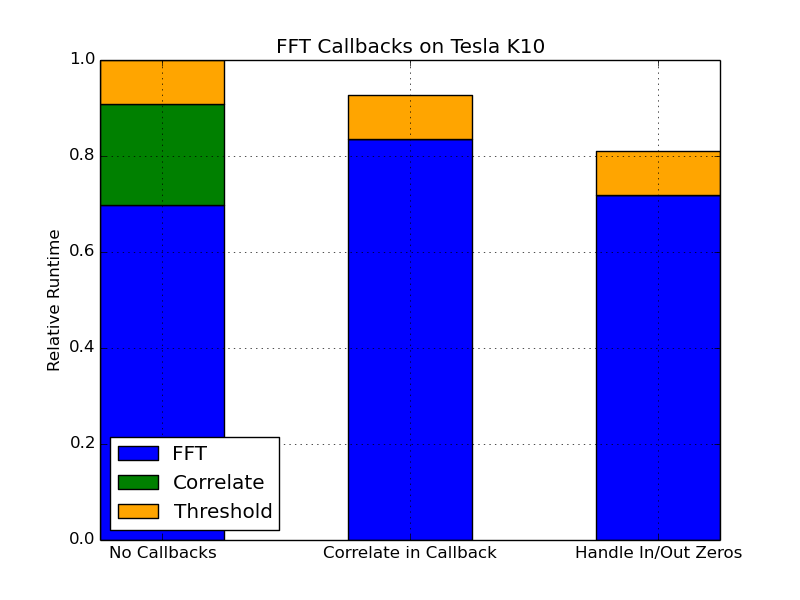
\includegraphics[width=0.6\textwidth]{papers/optimization/figures/callback.png}
\caption{\label{fig:callback} 
The relative performance of the kernels that make up the critical inner %loop of the 
matched-filtering code. Shorter bars represent better performance. Left: The initial GPU kernel implementations without the
use of cuFFT callbacks. Middle: Naive fusion of the correlate into a load callback.
Right: Fusion of the correlate kernel into the load callback, where memory reads
are avoided where the input is known to be zeros, and output writes are avoided
where it is known to be corrupted by wrap-around effects. It is not currently
possible to fuse the threshold kernel into the FFT, however we are working
with NVIDIA to make the necessary changes to the cuFFT callback API to further
optimize the code.
}
\end{figure}

More optimal use of the available memory bandwidth can also be achieved by
reducing the amount of data sent over the memory bus. We are investigating the
possibility of storing the output SNR time and input template phase as
half-precision (FP16) numbers to reduce memory bandwidth. We have also
discussed with NVIDIA the possibility of adding callbacks to the intermediate
steps of the cuFFT implementation (since our $2^{20}$ point FFTs are
implemented by three kernel calls in cuFFT) that would allow us to use FP16
precision between each FFT radix. Performing the FFT operations
in FP32 and storing the intermediate products in FP16 may be possible. We are beginning
a study to determine if this model could meet our accuracy requirements.

Finally, we are investigating the optimal GPU/CPU ratio for systems and
parellization between the host CPU and GPU kernel execution. As GPU kernel
launches are asynchronous compared to host execution, it is possible to hide
trivial serial operations that occur within the host code. The exception is
where triggers are offloaded from the GPU onto the CPU, which is a blocking
operation. Host execution does not proceed until the GPU queue is drained.
When the data is synchronized there is a noticeable delay before new GPU
kernels are executing. This can be minimized by executing multiple host
processes that submit work to the same GPU, and by batching additional work
together to amortize the device offload latency. We have shown that two
processes running on the same CPU launching kernels to a single GPU makes more
efficient use of the GPU resources; tests to find the optimal ratio are
ongoing.
